\documentclass{beamer}
%Information to be included in the title page:
\usetheme{default}
% \setbeamertemplate{background canvas}{\includegraphics
% 	[width=\paperwidth]{uclheader.pdf}}
	
% \definecolor{bluecolour}{rgb}{0.19,0.52,0.98}
% \useinnertheme[shadow=true]{rounded}
% \setbeamertemplate{items}[circle]
% \setbeamercolor{title}{bg=bluecolour, fg=black}
% \setbeamercolor{structure}{fg=bluecolour}

\title{Weekly meeting}
\subtitle{Meeting 2}
\date{31st October 2023}


\begin{document}

\frame{\titlepage}

\begin{frame}{Frame Title}
\frametitle{Table of Contents}
\tableofcontents
\end{frame}


\section{Progress and problems this week}
\begin{frame}{Progress this week}
    \begin{itemize}
        \item Ran simulations.py mostly successful.
        \item Set up Github repo
            \begin{itemize}
                \item I can share the link if that is useful.
            \end{itemize}
        \item Begun project outline
        \item Filled in risk assessment
            \begin{itemize}
                \item Very short, I think it needs to be signed by a supervisor before submitting. 
            \end{itemize}
        \item Read and skimmed through papers
    \end{itemize}
\end{frame}



\begin{frame}{Problems this week}
\begin{itemize}
    \item Attempted to run code
    \begin{itemize}
        \item Had some issues installing \emph{dmipy} package which I resolved
        \item It would be useful to have Snigdha's requirements file so that I know it will run correctly.
        \begin{itemize}
            \item I've switched to Python 3.8 and she is using 3.7, which didn't have a download link as it was no longer supported.
        \end{itemize}
        \item Had a run time error with the code that Snigdha shared.
            \begin{itemize}
                \item Switched \emph{num\_worker} from 2 to 0 and it ran. 
            \end{itemize}
        \item I can run 380 lines out of 400 before getting type errors when calculating the mean.
        \begin{itemize}
            \item I managed to get to this stage this afternoon, so haven't had the chance to resolve it yet. I think there's an issue with arguments in the numpy mean function.
        \end{itemize}
        \end{itemize}
    \end{itemize}
\end{frame}

\begin{frame}{Code figures}
\begin{figure} 
  \begin{minipage}[b]{0.4\linewidth}
  \centering
    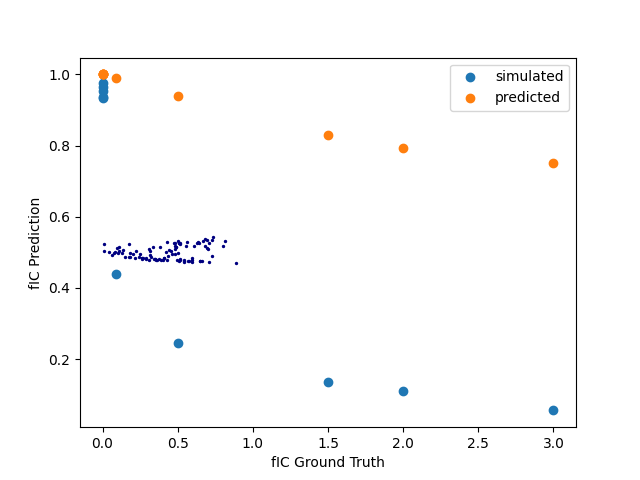
\includegraphics[width=\linewidth]{Weekly meeting slides/meeting 2/Figure_1.png} 
  \end{minipage} 
  \begin{minipage}[b]{0.4\linewidth}
  \centering
    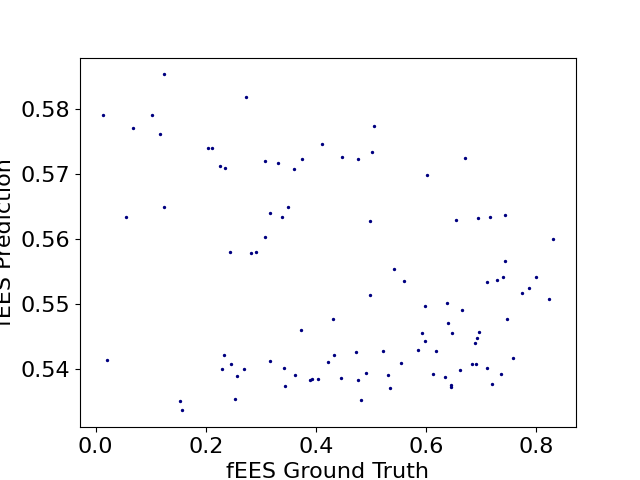
\includegraphics[width=\linewidth]{Weekly meeting slides/meeting 2/Figure_2.png} 
  \end{minipage} 
  \begin{minipage}[b]{0.4\linewidth}
  \centering
    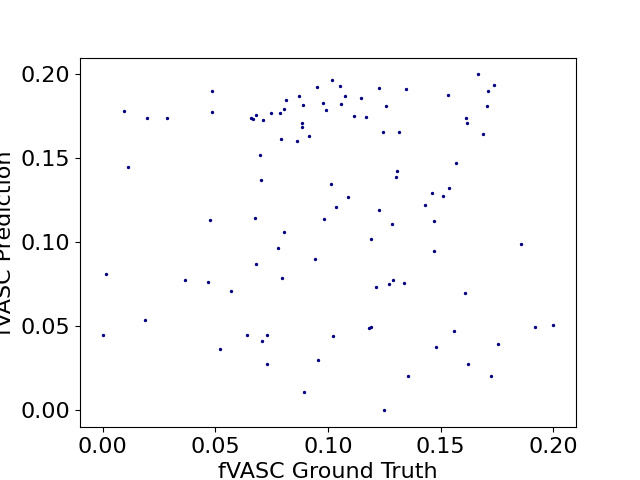
\includegraphics[width=\linewidth]{Weekly meeting slides/meeting 2/Figure_3.png} 
  \end{minipage} 
  \hfill
  \begin{minipage}[b]{0.4\linewidth}
  \centering
    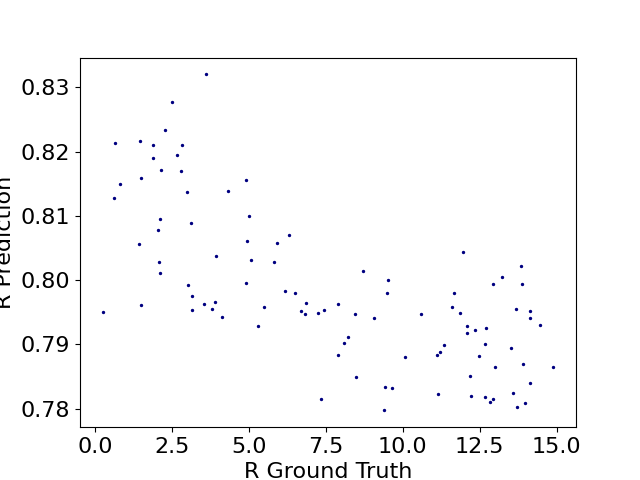
\includegraphics[width=\linewidth]{Weekly meeting slides/meeting 2/Figure_4.png} 
  \end{minipage} 
\end{figure}
\end{frame}

\begin{frame}{Code figures and error message}
  \begin{minipage}[b]{0.4\linewidth}
  \centering
    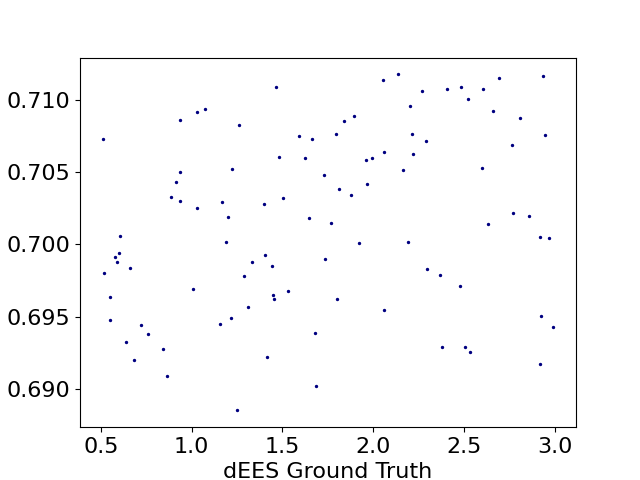
\includegraphics[width=\linewidth]{Weekly meeting slides/meeting 2/Figure_5.png} 
  \end{minipage} 
  \begin{figure}
      \centering
      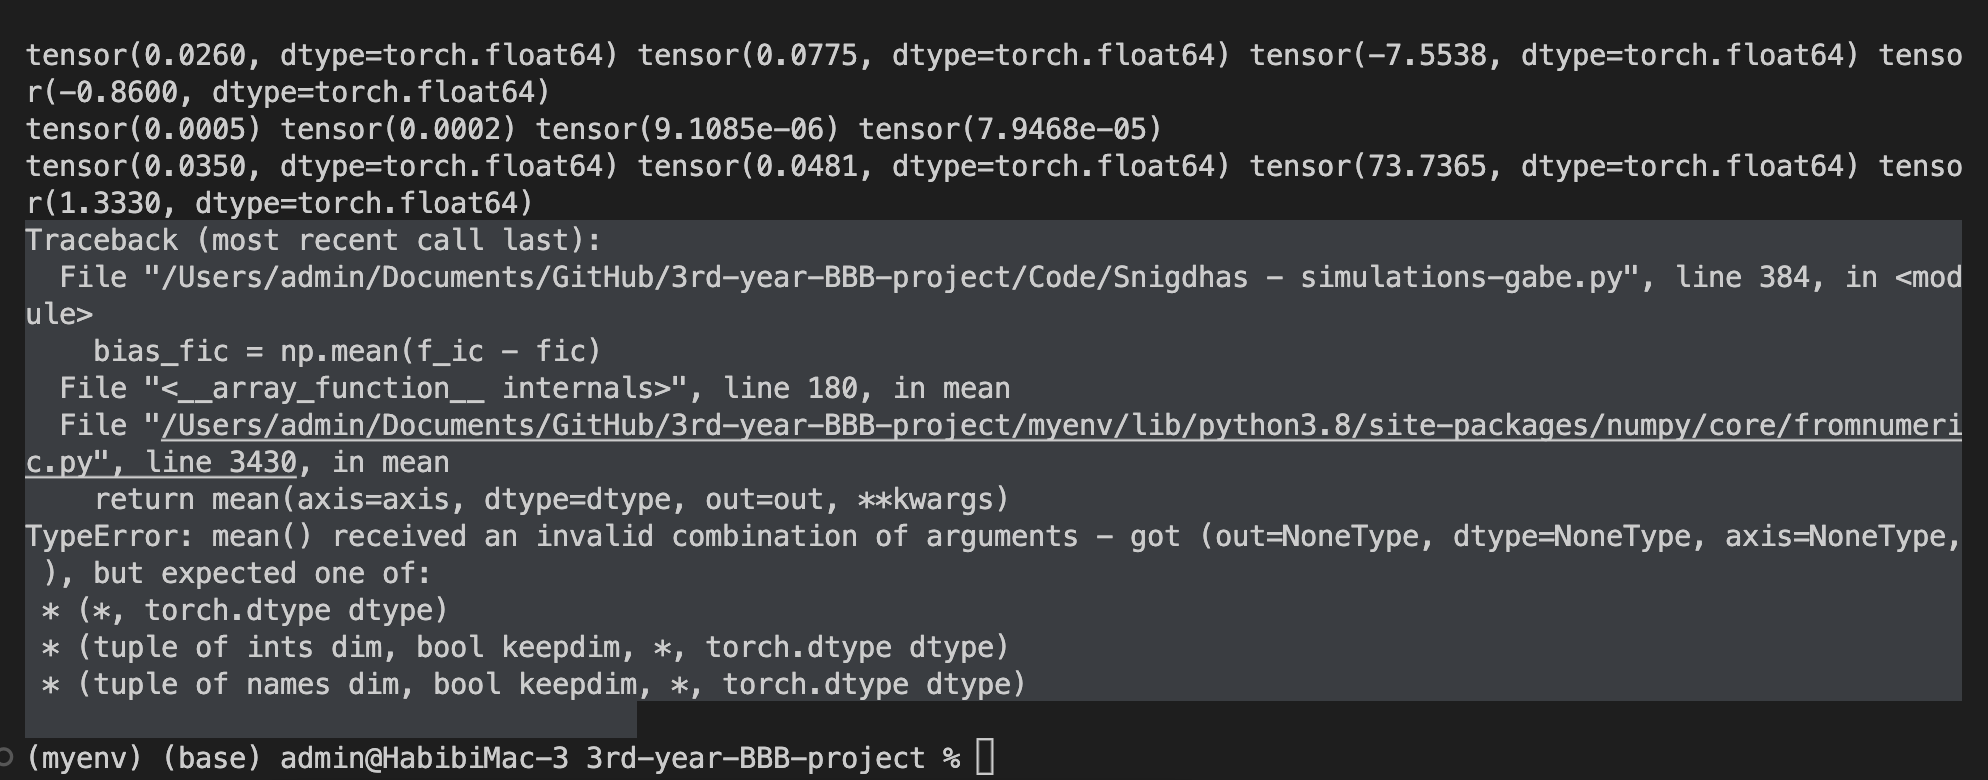
\includegraphics[width=\linewidth]{Weekly meeting slides/meeting 2/Screenshot 2023-10-31 at 1.46.04 pm.png}
      \label{fig:enter-label}
  \end{figure}
\end{frame}

\begin{frame}{Problems this week}
        \begin{itemize}
        \item How to read papers effectively?
        \begin{itemize}
            \item Which sections should I be focusing on?
            \item What is my goal when reading a paper?
        \end{itemize}
        \end{itemize}
\end{frame}

\begin{frame}{Problems this week}
    \begin{itemize}
        \item Github and Overleaf integration
        \item 
    \end{itemize}
\end{frame}

\begin{frame}{Answers from last week}
\begin{figure}
    \centering
    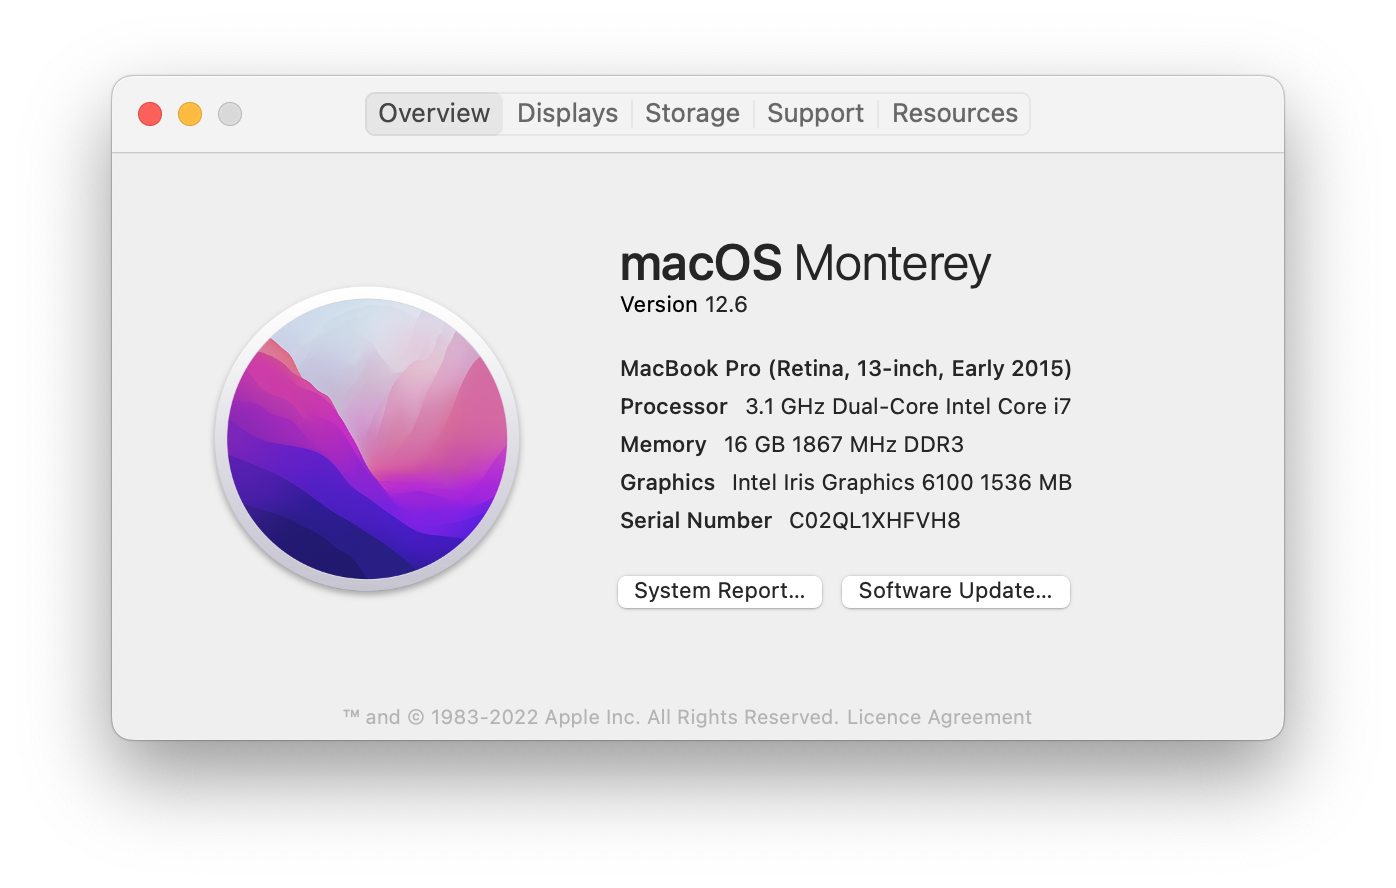
\includegraphics[scale=0.35]{Weekly meeting slides/meeting 2/Screenshot 2023-10-27 at 10.20.22 am.png}
    \label{fig:enter-label}
\end{figure}
\begin{itemize}
    \item Expected to spend 10-15 hours a week
\end{itemize}

\end{frame}

\section{Plan for next week}
\begin{frame}{Plan for next week}
    \begin{itemize}
    \item Project outline due on 3rd of November
    \begin{itemize}
      \item Create Gantt chart with main milestones of project
    \end{itemize}
    \item Sign off risk assesment
    \end{itemize}
\end{frame}

\section{Questions}

\begin{frame}{Questions}
    
\end{frame}

\end{document}